\chapter{The OpenCms module mechanism}
\label{The OpenCms module mechanism} 

%============================================================================

\section{Introduction to OpenCms modules}
OpenCms offers a module mechanism which provides an easy and convenient way to bundle and distribute templates 
and other functionality. A module usually consists of a set of templates, images, Java classes or libraries 
and other resources that depend on each other and thus should be distributed together.

This chapter provides an overview about the module installation process.
The full module documentation is available only in the interactive part of the OpenCms documentation.
This interactive documentation is of course packaged in modules, so to install the interactive 
documentation you first need to know how to install modules in Opencms.
This is why we have this chapter also here in the book part of the documentation.

Modules are managed in the OpenCms workplace in the Administration view under the option ``Module management". 
You can create, import, export or delete modules there. 
A module in a running system is a set of resources (folders and files) in the OpenCms VFS. 
If you export a module, all resources that belong to the module are written to a single ZIP file, 
including system settings required by OpenCms for the module to run.

You can import a module ZIP created this way in another OpenCms system with the module import option. 
The module ZIP file will then be unpacked and it's content will be copied to the specified location in the OpenCms VFS. 
Information about all installed modules is stored in the file \texttt{/WEB-INF/config/registry.xml}, 
located in the OpenCms servers web application context.

\section{How to import a module into OpenCms}

\begin{itemize}

\item Select {\em Administration} in the {\em View} selection of the workplace.
\begin{figure}[hbt]
\begin{center}
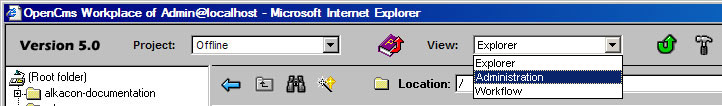
\includegraphics[width=\sgw]{pics/modules/import0}
\end{center}
\end{figure}

\item Select any ``offline" project (e.g. the default {\em Offline} project) in the {\em Project} selection:
\begin{figure}[hbt]
\begin{center}
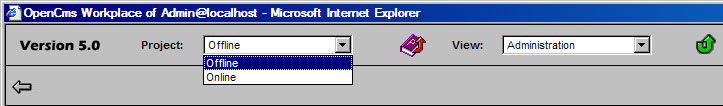
\includegraphics[width=\sgw]{pics/modules/import1}
\end{center}
\end{figure}

\item Open the {\em Module management}.

\item Click the {\em Upload module from} icon:
\begin{figure}[hbt]
\begin{center}
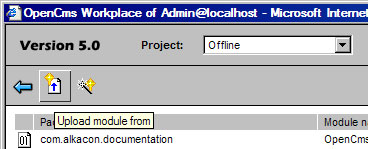
\includegraphics[width=\sgw]{pics/modules/import2}
\end{center}
\end{figure}

\item The module import wizard starts. On the first page of the wizard you can choose from where you want 
to upload the module's zip file:
\begin{figure}[hbt]
\begin{center}
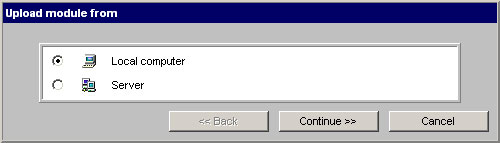
\includegraphics[width=\sgw]{pics/modules/import3}
\end{center}
\end{figure}

\begin{itemize}

\item {\em Local computer}: use this option to upload the module anywhere from your local filesystem 
(using http upload). On the next wizard page a file search dialog is shown and you can select the 
module's zip file in the local file system of your computer. 

\item {\em Server}: use this option to upload the module from the {\tt WEB-INF/export/modules/} directory of 
your OpenCms web application on the server.
On the next wizard page you get a selection with the package names of all modules found in 
{\tt WEB-INF/export/modules/} to choose from. 

\end{itemize}

\item Finally, click {\em Continue}. The import starts, reporting which files and folders are imported.

\item You might get an error or exception message during the import that tells you that you should do a 
restart afterwards. If so, do what you are told, and restart the OpenCms server after the last step. Be 
aware that you might have to restart the OpenCms server even if no such message is shown, see below for 
more details.

\item After you have left the import dialog the wizard ends and you should find the imported module in 
the list of all modules. 

\end{itemize}

\subsection{Restarting the OpenCms server after module import}

A server restart {\em might} be required after you imported a new (or updated) module.

Some modules contain Java archives (JARs), class files or other resources that are automatically 
copied to the WEB-INF/classes/ or WEB-INF/lib/ folder of the OpenCms web application during the module import. 
Such modules sometimes require a restart of the OpenCms Servlet container so that the Java Classloader can 
load these new classes or resources.

The individual module documentation should contain a note if a module requires a server restart after 
installation. You will {\bf not} always get an exception message during import if the module requires a server 
restart. 

In case you upload several modules, one server restart is usually enough after uploading all modules.

\section{How to create, administrate, replace and export a module}

For a detailed description about the

\begin{itemize}

\item creation of a new module

\item administration of an existing module

\item replacement of an existing module with a new version (i.e. updating)

\item distribution of a module with the export function 

\end{itemize}

please import the OpenCms interactive documentation module

{\tt com.alkacon.documentation.documentation-modules}.

See chapter \ref{About this documentation} on how and where to obtain this module.